\chapter{Vlastní řešení}  

V této části navrhneme podobu vlastního řešení problému specifikovaného v předchozích kapitolách. 

\section{Návrh}

Tato práce se zaobírá webovou službou, která bude poskytovat svoje rozhraní a funkcionalitu portálům Moodle a CourseWare. Jedná se o jednoduchou aplikaci s jediným účelem, tedy kompilace \LaTeX\ souborů do PDF. Tudíž není potřeba ani persistentní vrstvy, výsledný soubor PDF bude uložen do klasického souborového systému. 

\subsection{Platforma}
Na základě požadavků bude aplikace postavena na Java EE, což je platforma pro vývoj webových aplikací, rozšiřující standardní Javu SE. O proti ní poskytuje některé zásadní techniky navíc, jednu se tedy představme. 
\par
\textbf{Vkládání závislostí} (dependency injection) umožňuje objektu používat jiné objekty bez potřeby ho zatěžovat jejich vytvářením. Obekty, které můžeme takto vkládat se nazývají beany a právě o jejich vytváření a zánik se stará Contexts and Dependency Injection(dále jen CDI) kontejner.
\\[12pt]
\par
Dále je potřeba specifikovat aplikační server, ten poskytuje pro webové aplikace běhové prostředí, tedy zajišťuje správu databázových spojení apod. Na základě zkušeností je vybrán open-source Payara, který staví na GlassFish, o proti němu poskytuje častější aktualizace a opravy chyb. 

\subsection{Komunikace}
Pro komunikaci mezi klientem a serverem je vybráno REST Api. Poskytuje jednoduché rozhraní s kterým je schopen komunikovat jakýkoliv systém pouze za znalosti struktury požadavků a odpovědí. Posílání zpráv bude postaveno nad protokolem HTTP pomocí GET a POST metod. Na obrázku \ref{fig:seq} je zobrazena komunikace mezi serverem a klientem. 

\begin{figure}[H]
	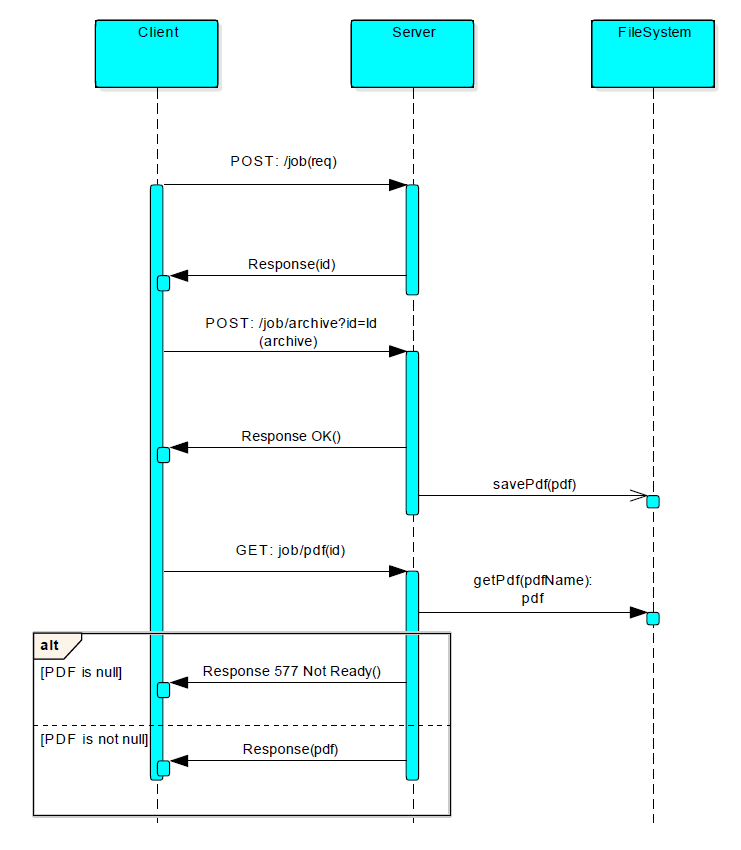
\includegraphics[width=0.9\textwidth]{diagram}
	\centering
	\caption{Sekvenční diagram}
	\label{fig:seq}
\end{figure}

Kompletní dokumentace k rozhraní se nachází na https://app.swaggerhub.com/apis/Tadky/Thesis/1. Na ukázku vypíšeme alespoň používané zdroje:
\begin{itemize}
	\item \textbf{POST} {\ttfamily /job?token=<clientToken>} - Slouží k předání požadavků na výsledné PDF.
	\item \textbf{POST} {\ttfamily /job/archive?id=<jobId>\&token=<clientToken>} - Musí obsahovat zip archiv s potřebnými soubory pro kompilaci.
	\item \textbf{GET} {\ttfamily /job/pdf?id=<jobId>\&token=<clientToken>} - Vrací výsledné PDF, pokud už je hotové.
\end{itemize}

Autentizace bude probíhat skrz tokeny, které budou mít dané portály vygenerované a budou se nimi ověřovat.

\subsection{Kompilace}
Pro vytvoření PDF je potřeba příslušně zkompilovat celý \LaTeX\ projekt 
Na základě porovnání kompilátorů(3.3) z předchozí kapitoly je zvolen MikTeX, který poskytuje vše potřebné a nabízí vhodné funkcionality pro téma této práce např. doinstalovávání balíčku za běhu. 

Jelikož jsou kladeny požadavky na výsledný soubor PDF a bohužel kompilátory tyto úpravy nepodporují je potřeba použít jiný nástroj, který bude umožňovat měnit soubor podle požadavků. Nejvíce vhodný se zdá PDFtk\footnote{https://www.pdflabs.com/tools/pdftk-server/}, který je pod GPL licencí a nabízí vše potřebné. 

\subsection{Server}




